\section{GNOME Project Analysis} % {{{

\marginnote{
\includegraphics[width=\marginparwidth]{gnome/logo}}

GNOME is a desktop environment for \textsmaller{UNIX} based systems. It
is composed by a collection of tools and programs including a desktop shell in
order to provide all the essential utilities a user might need when working
with a computer. Officially, GNOME is part of the \ac{GNU} project and licensed
under the \ac{GPL} and the \ac{LGPL}. The name GNOME was initially an acronym
for \emph{GNU Network Object Model Environment}, however that acronym was
dropped. The GNOME project targets ease of use and user friendliness and
therefore aims for coherent and good user interfaces \cite{GNOMEHIG},
accessibility, internationalization, regular releases and good support for
users and developers. GNOME is a modular project, meaning that it consists of
several so called modules, which can be either applications, libraries or
utilities. Since the release of GNOME~3, the modules were reorganized into a
GNOME Core suite and a GNOME Apps suite. GNOME Core provides everything to run
a basic desktop system and will therefore be analyzed in this context.

\subsection{History} % {{{

GNOME was first announced and started in 1997 by Miguel de Icaza and Federico
Mena Quintero as a counterpart to KDE
\cite{German2003,GNOMEAbout,GNOMEAnnouncement}. Both were university students
at the time when they set their aim to produce a desktop environment using only
free software technologies. KDE relied on the Qt widget toolkit, which at the
time was licensed under a proprietary software license. Instead of using Qt,
they used the \ac{GTK} originally developed for the \textsmaller{GIMP} graphics
editor. The GNOME project quickly grew into a large project which nowadays is
the most popular desktop environment for \textsmaller{UNIX} type operating
systems. The desktop as well as the developer technologies can be found on
workstations and large enterprises but also on mobile devices. With the recent
GNOME~3 release a major overhaul with a significant redesign of the desktop
environment and an entirely new user interface took place \cite{GNOMEPress}.

\begin{figure}[htbp]
  \centering
  \includegraphics[width=0.8\textwidth]{gnome/commits_by_author}
  \caption[Commits by Most Active Authors, GNOME]
  {Monthly activity of the most active GNOME Core developers. The
    disproportional amount of commits by Matthias Clasen can be interpreted
    with a high skill set and lots of effort he puts in the project.}
  \label{fig:gnome:cba}
\end{figure}

% }}}

\subsection{Community} % {{{

The GNOME project consists of a large user and developer community. While there
were about 3500 people contributing to GNOME and its applications, there is
also a big community around the project, which for example uses GNOME
technologies such as GStreamer or \ac{GTK} \cite{GNOMEAbout,GNOMETeams}.

Most of the communication inside the project is handled through mailing lists
and \ac{IRC} channels. Almost every GNOME module has a dedicated mailing list
or \ac{IRC} channel. Global decisions are mostly handled through the
\emph{desktop-devel} mailing list. Additionally blogs are widely spread in the
GNOME community and contributors often write blog posts about achievements,
wishes or start discussions.

Next to several hackfests each year, the community holds a yearly conference
under the name \textsmaller{GUADEC}. It stands for GNOME User and Developer
European Conference, and while the conference only took place in Europe so far
it is nevertheless considered worldwide by the community \cite{GNOMEGUADEC}.

\begin{table}
  \centering
  \begin{tabularx}{\textwidth}{lXr}
    \toprule
    \tableheadline{Event}                   & \tableheadline{Venue}       & \tableheadline{Date} \\
    \midrule
    GUADEC \MakeUppercase{\romannumeral 1}  & Paris, France               & 2000 \\
    GUADEC \MakeUppercase{\romannumeral 2}  & Copenhagen, Denmark         & 2001 \\
    GUADEC \MakeUppercase{\romannumeral 3}  & Seville, Spain              & 2002 \\
    GUADEC \MakeUppercase{\romannumeral 4}  & Dublin, Ireland             & 2003 \\
    GUADEC \MakeUppercase{\romannumeral 5}  & Kristiansand, Norway        & 2004 \\
    GUADEC \MakeUppercase{\romannumeral 6}  & Stuttgart, Germany          & 2005 \\
    GUADEC \MakeUppercase{\romannumeral 7}  & Vilanova i la Geltrú, Spain & 2006 \\
    GUADEC \MakeUppercase{\romannumeral 8}  & Birmingham, England         & 2007 \\
    GUADEC \MakeUppercase{\romannumeral 9}  & Istanbul, Turkey            & 2008 \\
    Desktop Summit                          & Gran Canaria, Spain         & 2009 \\
    GUADEC \MakeUppercase{\romannumeral 10} & The Hague, Netherlands      & 2010 \\
    Desktop Summit                          & Berlin, Germany             & 2011 \\
    GUADEC \MakeUppercase{\romannumeral 11} & La Coruña, Spain            & 2012 \\
    \bottomrule
  \end{tabularx}
  \caption[Previous and Planned GNOME Conferences]{Previous and planned GNOME conferences.}
\end{table}

Due to the large and modular composition of the GNOME project, there are
similar roles for each module. Only very few teams and roles stand above all
modules. In this respect the developer community can be very much be seen as a
flat structure \cite{GNOMETeams,German2003,GNOMEDesignTeam,GNOMEReleaseTeam}.

\paragraph{Committer}

Any person who contributed a reasonable amount of improvements to the GNOME
project or to a single module can become a committer. A committer has full read
and write access to all GNOME repositories. Each commit will however be
reviewed and approved by the maintainer of the module. To get such an account,
one has to make a formal request to the accounts team along with one or several
vouchers who can confirm ones contributions to the GNOME project. Every module
maintainer or translation team leader can act as a voucher. Furthermore the
voucher will be responsible for the actions of the requesting person on the
repositories.

\paragraph{Maintainer}

Every module has one or more maintainers who will be responsible for releases,
reviewing patches and the direction of a module. They are the main contact for
the community and therefore act as the leader of a certain module. A single
module can be maintained by multiple maintainers and one maintainer can
maintain several modules. To become a maintainer one has either to create a new
module which gets incorporated into the GNOME project or be asked by another
maintainer.

\begin{figure}[htbp]
  \centering
  \includegraphics[width=0.8\textwidth]{gnome/commits_by_year}
  \caption[Commits by Year, GNOME]
  {Yearly overview of commits to GNOME Core. The leap in 2008 appears to be
    related to GNOME~2.22 or GNOME~2.24.}
  \label{fig:gnome:cby}
\end{figure}

\paragraph{Release Team}

This team is responsible for a wide range of tasks concerning the development
process of the GNOME project. Their tasks include for example creating a
development schedule, making and publishing releases, approving or rejecting
freeze break requests and defining the module list for GNOME releases. The team
size is not fixed and can vary over time. Membership is only by invitation and
often only when one person leaves the team to free up one space. The leaving
person may recommend a new team member which the team will decide upon.

\paragraph{Design Team}

Since GNOME~3 the design team holds a much more important role in the GNOME
project as they primarily define the design of the GNOME user experience. This
is done by designing the user interface and workflow of GNOME modules.
Additionally they play an important part in the feature based development
process.

\paragraph{GNOME Founders}

Miguel de Icaza and Federico Mena Quintero, the original GNOME founders, played
an important role in the first years of the GNOME project. Nowadays however
they are more active in projects around GNOME technologies and often act as
visionaries.

% }}}

\subsection{Release Process} % {{{

\begin{figure}[htbp]
  \centering
  \includegraphics[width=\textwidth]{gnome/releases}
  \caption[Major Releases of GNOME]{Major releases of GNOME.}
\end{figure}

\begin{figure}[hbtp]
  \centering
  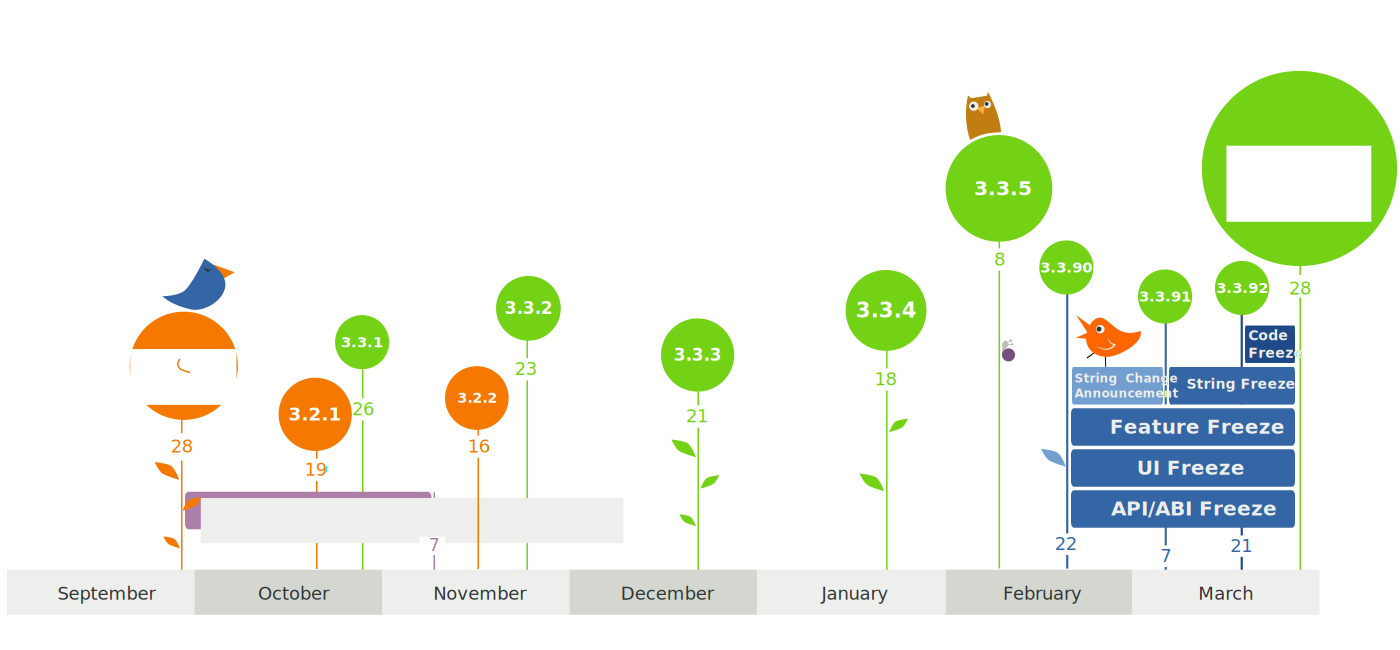
\includegraphics[width=0.95\textwidth]{gnome/gnome-timeline}
  \caption[GNOME 3.4 Release Schedule]{Release schedule which will lead to GNOME 3.4.}
\end{figure}

The GNOME project uses a versioning scheme with three numbers however
distinguishes only between major and minor releases
\cite{GNOMEDevelopmentSchedule,GNOMESchedule}. The numbers are however
nevertheless called major, minor and micro numbers. An incrementation of the
first number only occurs when the project does a ground-breaking change, such
as using \ac{GTK}+2 for GNOME~2.x or the new user experience with the GNOME shell
and \ac{GTK}+3 for GNOME~3.x. For the minor version number the GNOME project uses
odd numbers indicating an unstable series and even numbers for stable releases.
For example the unstable 3.1.x series will become the stable 3.2.x release
series.

The release schedule is fixed with a new major release appearing every six
months. To achieve this, the release team publishes a release schedule in the
same frequency \cite{GNOMEDevelopmentSchedule}. Over the years it stayed mostly
the same, while few minor changes may occur to comprise conferences or
holidays. The release schedule includes future stable minor releases, the two
schedules overlap.

Each stable release series consists of at least three releases which are named
with x.y.0 to x.y.2. Of course, a module maintainer can decide to provide more
stable releases \cite{GNOMEReleaseTeam}. The unstable series consists of eight
releases which are distributed over six months. The schedule furthermore
includes proposal and freeze periods which will be described in the following
\cite{GNOMEDevelopmentSchedule,GNOMESchedule}.

\begin{figure}[bhtp]
  \centering
  \includegraphics[width=\textwidth]{gnome/punchcard}
  \caption[Time Based View on Commits, GNOME]
  {Time based view on commits of core contributors. It seems that most
    developers are employed. The high number on Monday can be explained with
    the release preparation which are always done on Monday evening.}
  \label{fig:gnome:p}
\end{figure}

\begin{figure}[htbp]
  \centering
  \includegraphics[width=0.8\textwidth]{gnome/commits_by_month}
  \caption[Commits by Month, GNOME]
  {Amount of commits per month of core contributors. The project quite shows a
    linear growth with peaks every six months.}
  \label{fig:gnome:cbm}
\end{figure}

\paragraph{Feature proposal period}

After a major release gets published the feature proposal period starts. GNOME
developers can propose features for the next major release and discuss them
with the community. Approximately a month later, when the first unstable
release gets published, the proposal period ends. Around two weeks later the
release team meets and decides about proposed features with the community input
given up to this point.

\paragraph{The Freeze}

With the first beta released the first freeze takes action. No user interface
changes, new features or developer \ac{API} changes are allowed without
approval from the release team. This excludes of course bug fixes. Additionally
new translatable strings must be announced to the translation and documentation
team.

\paragraph{String Freeze}

With the second beta release no string changes are allowed anymore without
confirmation of both the release and translation team.

\paragraph{Hard Code Freeze}

With the release of the release candidate no source code changes are allowed
without approval of the release team. Documentation and translation however can
continue. After publishing the next major GNOME release the Hard Code Freeze
ends but all other freezes remain in action for the stable series.

\begin{figure}[htbp]
  \centering
  \includegraphics[width=0.8\textwidth]{gnome/authors_by_month}
  \caption[Authors by Month, GNOME]
  {Amount of distinct authors of GNOME Core over time. Especially the
    development of GNOME~3 which started in 2010 appears to have attracted
    additional developers.}
  \label{fig:gnome:abm}
\end{figure}

% }}}

\subsection{Development} % {{{

Before the release of GNOME~3, the release team together with the community
decide about the inclusion of new modules. The development of each module was
planned and executed by the maintainers. Since GNOME~3, the development
workflow changed into a more design driven development approach. This means
that all new features concerning user interfaces or applications have to go
through the design team \cite{GNOMEDesignTeam}. This leads to a consistent
process with a uniform user interface. However the design team has no decision
making authority and a maintainer can ignore the design team's proposal.

Next to the design driven approach the module inclusion changed to a feature
inclusion approach \cite{GNOMEFeatures3.4,GNOMERoadMap}. Every GNOME
contributor can create a feature proposal in which one describes a feature they
would like to see in the next stable GNOME release. A feature proposal is
composed by a description of the problem which will be solved, one or more
authors, a list of involved parties and the current state of the proposal. All
of these fields are required and a feature will not be accepted until all are
completed. After each major release and until about a month later, one can
propose a feature for inclusion. The community has time to discuss the features
and improve them for roughly one and a half months. After that time the release
team will meet and depending on the feedback of the community decide about the
inclusion of each feature. If a feature gets accepted the author of the feature
will be its leader and responsible for the completion. With the release of the
first beta release and the establishment of the Feature, \ac{UI} and
\ac{API}/\acs{ABI} Freeze the feature has to be finished and working. If not,
it may be postponed to the next major release.

% }}}

% }}}
